% \documentclass{cmspaper}
%\begin{document}

\section{Electron Studies} \label{sec:electrons}

\subsection{Identification and Isolation} \label{sec:IdAndIso}

A reconstructed electron object is formed from deposition of energy in ECAL (called a ``supercluster'') 
that has an extrapolated track pointing to it. This study uses the standard ``GsfElectron'' 
collection of MC events~\cite{Baffioni:934070}.
The reconstruction algorithm of Ref \cite{Baffioni:934070} first matches the 
supercluster to hits in the pixel detector.
The pixel hits are then used to seed a track.  Finally, a track is fitted to all hits using the Gaussian Sum Filter 
(GSF) algorithm, which reconstructs the track to the ECAL surface
despite the possible presence of kinks from electron bremsstrahlung.  
The $p_{T}$ and $\eta$ of the electrons are calculated using both calorimeter and tracker information, 
taking account of detector resolutions and its dependence on $p_{T}$.
Standard CMS corrections are applied to set correctly the electromagnetic (EM) energy scale.

%#######Ref for CMSSW electron energy scale #############

%that is matched with hits in the pixel detector.  Few electrons loose momentum to radiated photons before the pixel detector since the majority of the material in the tracker is after the pixels.  Thus, the energy-weighted average impact point of the electrons and radiated photons with the supercluster will correspond well with the track found using these pixel hits as seeds.  

The criteria used for electron identification (ID) at the reconstruction level are very loose, thereby contributing many false electrons 
to the collection. In this analysis, the HEEP selections for electron ID and isolation~\cite{HEEPNOTE}, which are optimized for 
electrons with energies of hundreds of GeV, have been applied in an effort to: i) keep the efficiency high for electrons 
from LQ decays that have high $p_{T}$, and ii) reduce the number of jets mimicking electrons.
The definitions of the variables used in this analysis are given below:
%
\begin{itemize}
%
\item $H/E$: the ratio of the energy in all the HCAL RecHits within a radius of 0.1 to 
the electromagnetic energy of the supercluster associated with the electron; 
an H/E cut of $<0.1$ is applied at pre-selection level.
%
\item $\sigma_{\eta\eta}$: a variable reflecting the distribution along $\eta$ of the electron shower 
\begin{displaymath}
\sigma_{\eta\eta} = \frac{\sum_k^{5x5} w_k( i_{\eta}^k - \bar{i_{\eta}} )^2 \quad}{\sum_k^{5x5} w_k} \quad ,
\end{displaymath}
where $i_{\eta}^k$ is the index of the $\eta$ position of the $k^{th}$ crystal in a 5x5 matrix 
of crystals centered on the seed crystal of the cluster associated to the electron, 
$\bar{i_{\eta}}$ is the energy weighted mean index of the $\eta$ position of the 5x5 block, 
and $w_k$ is a weight given to each crystal as defined by
\begin{displaymath}
w_k = 4.2 + ln (\frac{E_k}{E_{5x5}}) \quad , 
\end{displaymath}
where $E_k$ is the energy of the $k^{th}$ crystal and $E_{5x5}$ is the total energy deposited in the 5x5 block.
The values for the endcap are corrected for the different crystal size with respect to the barrel region.
%sqrt(sigEtaEta) - 0.02 (abs(eta) - 2.3)
%http://cmssw.cvs.cern.ch/cgi-bin/cmssw.cgi/CMSSW/RecoEcal/EgammaCoreTools/src/EcalClusterTools.cc?revision=1.14&view=markup&pathrev=V00-05-18%
%
\item $\Delta\eta^{trk-SC}$ and $\Delta\phi^{trk-SC}$: the difference in $\eta$ and $\phi$ between the track position extrapolated from 
the inner layer tracker to the ECAL surface and the $\eta$ and $\phi$ of the supercluster.
%
\item Number of Tracks ($N_T$): with $p_{T}>1.5$ GeV in an annulus $0.02 < \Delta\mbox{R} < 0.2 $ around the direction of the electron;
%
\item Track Isolation (Track Iso): the sum of the $p_{T}$ of tracks in the annulus defined above for $N_T$.
%
%
\item EM Isolation (Iso): the transverse part of the electromagnetic energy 
of all the ECAL Rec Hits (energy deposits in single channels)
%deposited in all the clusters 
in a cone $\Delta\mbox{R} < 0.3$, 
centered on the electron's position in the calorimeter, excluding the Rec Hits that make up the supercluster;
%
\item HAD Isolation: the transverse part of the hadronic energy of all the HCAL Rec Hits in an annulus
$0.15 < \Delta\mbox{R} < 0.3$, centered on the electron's position in the calorimeter. 
%
\end{itemize}

Figures~\ref{fig:elecID} and~\ref{fig:elecIso} show, respectively, distributions of ID and Isolation variables, 
for both true electrons from LQ decays and fake electrons from a sample of QCD multi jet events. 
Table~3 
%\ref{tab:HEEPselection} 
summarizes the HEEP selection used in this analysis. 

Recently, HEEP ID and Isolation criteria have been improved
and some new reconstructed variables are available in the latest version 
of the CMS analysis software. 
%leading to a better rejection of jets mimicking electrons, 
%while keeping the same efficiency on true electrons. 
The impact of this improvement will be investigated in 
future upgrades of this analysis. 

%From : twiki.cern.ch/twiki/bin/view/CMS/SWGuideEgamma

% Robust Electron Def from : twiki.cern.ch/twiki/bin/view/CMS/SWGuideElectronID
% Ele Isolation from : twiki.cern.ch/twiki/bin/view/CMS/SWGuideEgamma 

%Still need description of these plots, like what cuts were used...

%\begin{2figures}{hbtp}
%  \resizebox{\linewidth}{!}{\includegraphics{plots/h_eleDeltaEtaTrkSC.eps}} &
%  \resizebox{\linewidth}{!}{\includegraphics{plots/h_eleDeltaPhiTrkSC.eps}} \\
%  \caption{eleDeltaEtaTrkSC}
%  \label{fig:eleDeltaEtaTrkSC} &
%  \caption{\small \sl eleDeltaPhiTrkSC}
%  \label{fig:eleDeltaPhiTrkSC} \\
%\end{2figures}
%\begin{2figures}{hbtp}
%  \resizebox{\linewidth}{!}{\includegraphics{plots/h_eleHoE.eps}} &
%  \resizebox{\linewidth}{!}{\includegraphics{plots/h_eleSigmaEE.eps}} \\
%  \caption{\small \sl eleHoE}
%  \label{fig:eleHoE} &
%  \caption{\small \sl eleSigmaEE}
%  \label{fig:eleSigmaEE} \\
%\end{2figures}
%\begin{2figures}{hbtp}
%  \resizebox{\linewidth}{!}{\includegraphics{plots/h_eleNumTrkIso.eps}} &
%  \resizebox{\linewidth}{!}{\includegraphics{plots/h_eleEcalIso.eps}} \\
%  \caption{\small \sl eleNumTrkIso}
%  \label{fig:eleNumTrkIso} &
%  \caption{\small \sl eleEcalIso}
%  \label{fig:eleEcalIso} \\
%\end{2figures}
%\begin{figure}
%  \begin{center}
%    \resizebox{0.5\linewidth}{!}{\includegraphics{plots/h_eleTrkIso.eps}}
%    \caption{\small \sl eleTrkIso}
%    \label{fig:eleTrkIso}
%  \end{center}
%\end{figure}

\begin{figure}
  \begin{center}
  \begin{tabular}{cc}
  \resizebox{7cm}{!}{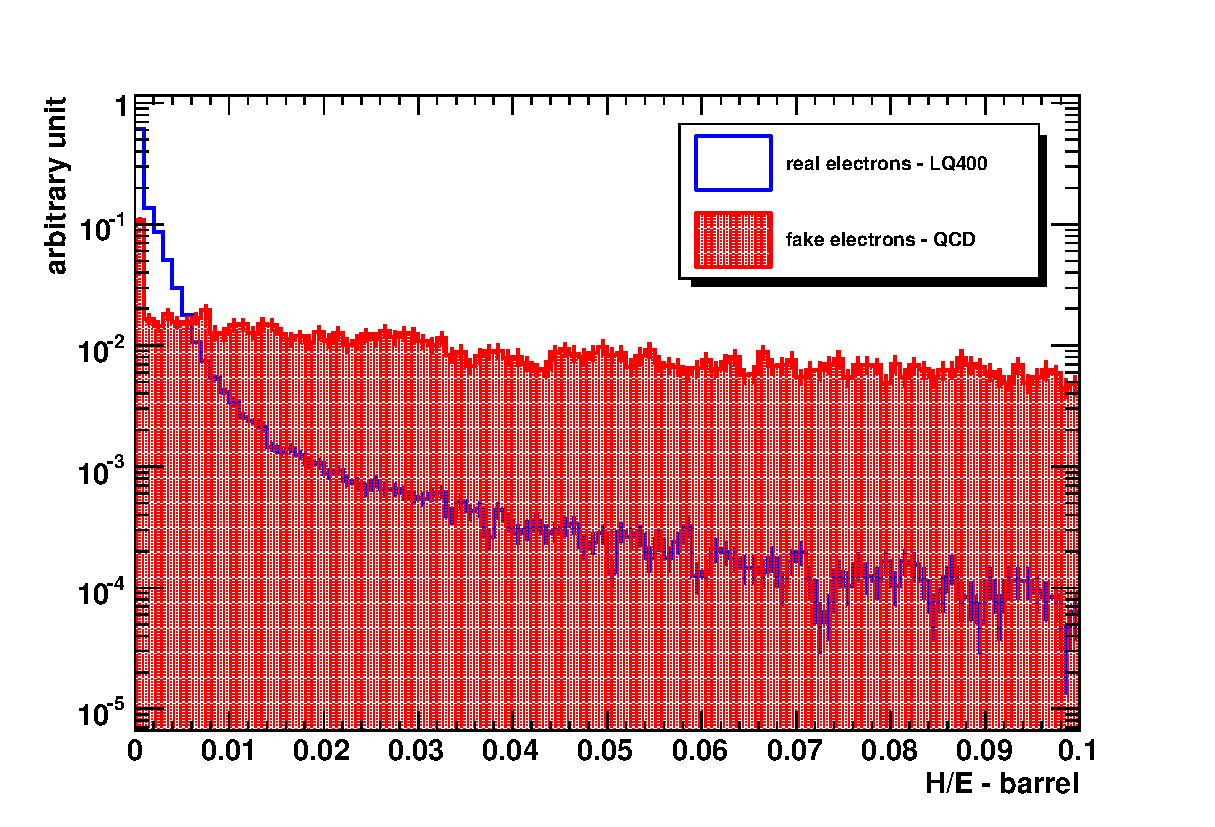
\includegraphics{plots/electronStudies/eleHoE_barrel_LQ400vsQCD.eps}} &
  \resizebox{7cm}{!}{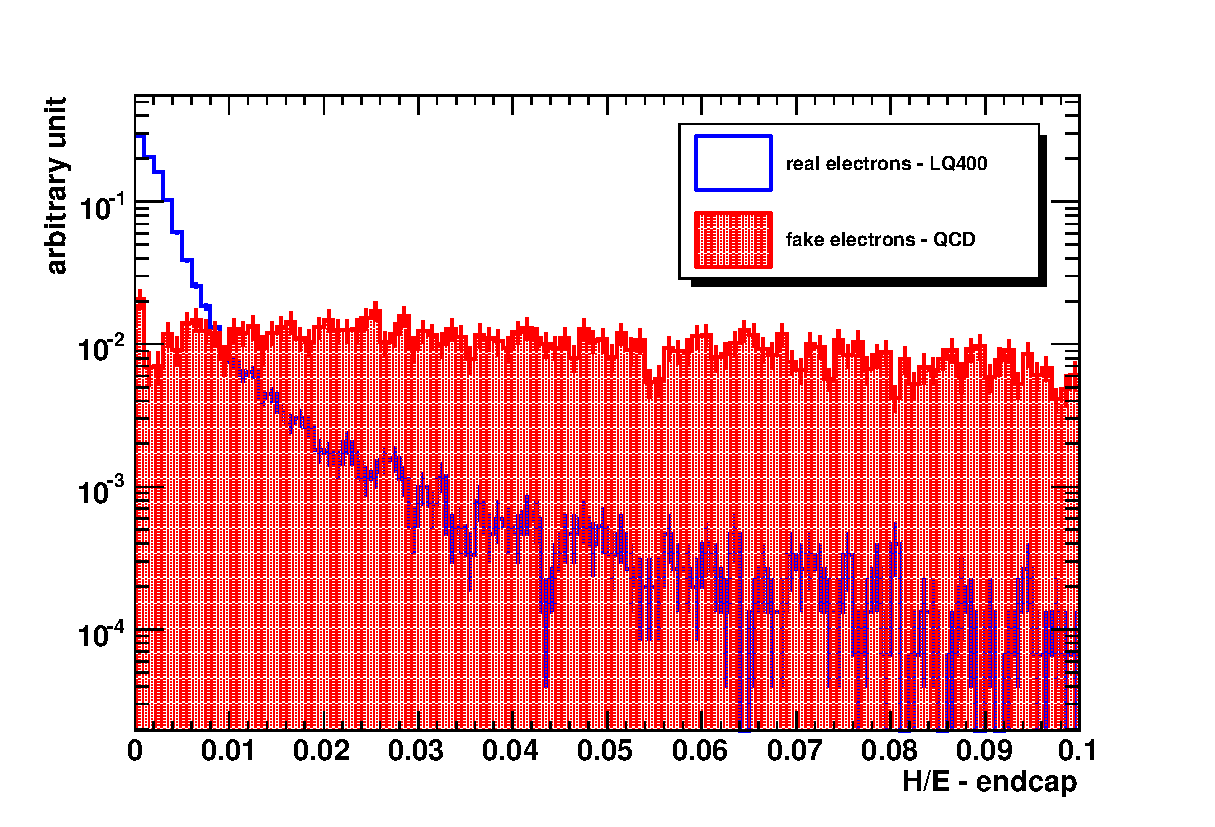
\includegraphics{plots/electronStudies/eleHoE_endcap_LQ400vsQCD.eps}} \\
  \resizebox{7cm}{!}{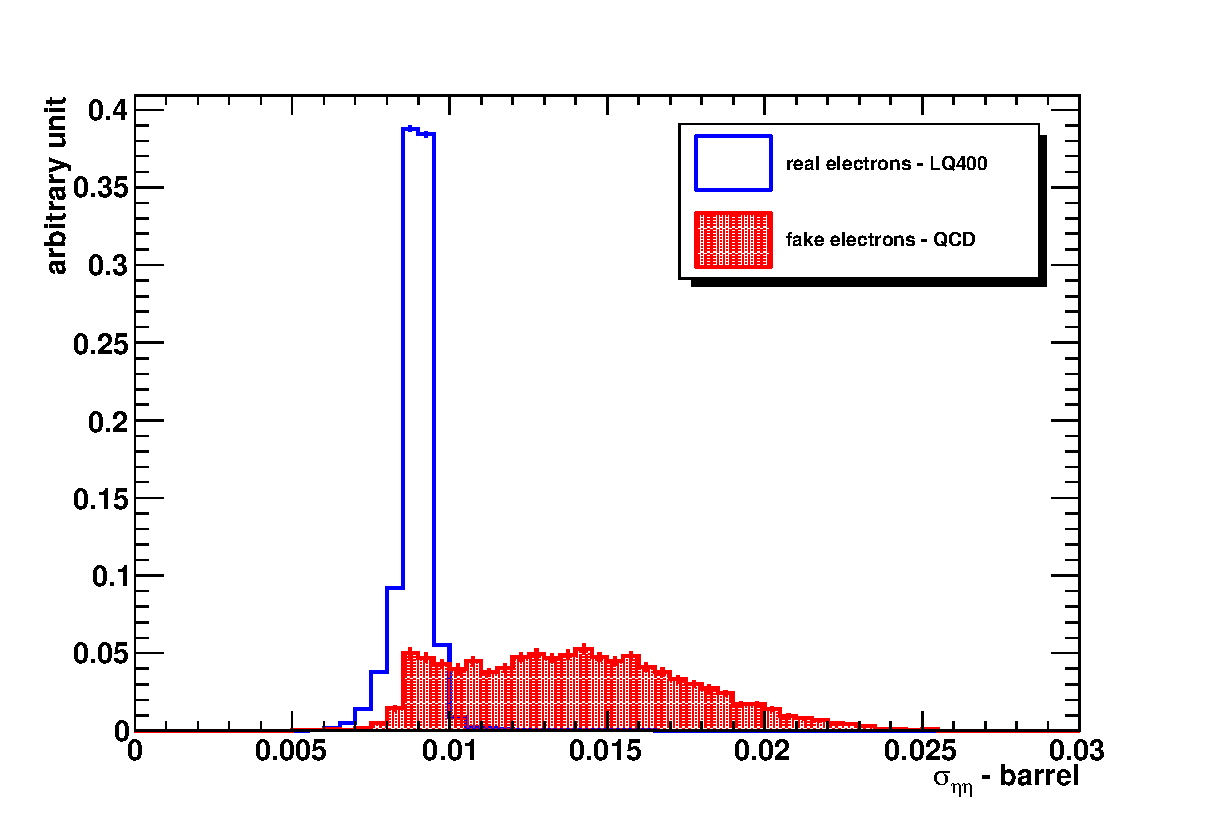
\includegraphics{plots/electronStudies/eleSigmaEE_barrel_LQ400vsQCD.eps}} &
  \resizebox{7cm}{!}{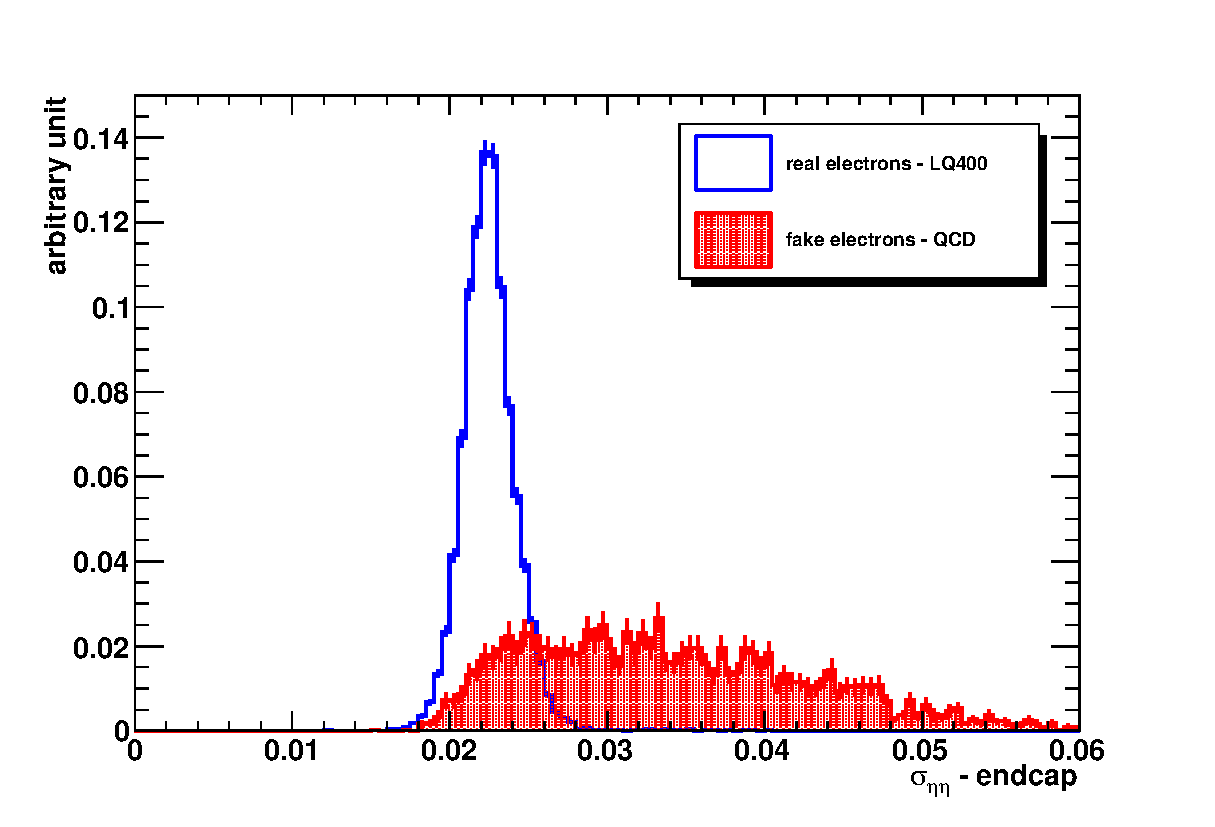
\includegraphics{plots/electronStudies/eleSigmaEE_endcap_LQ400vsQCD.eps}} \\
  \resizebox{7cm}{!}{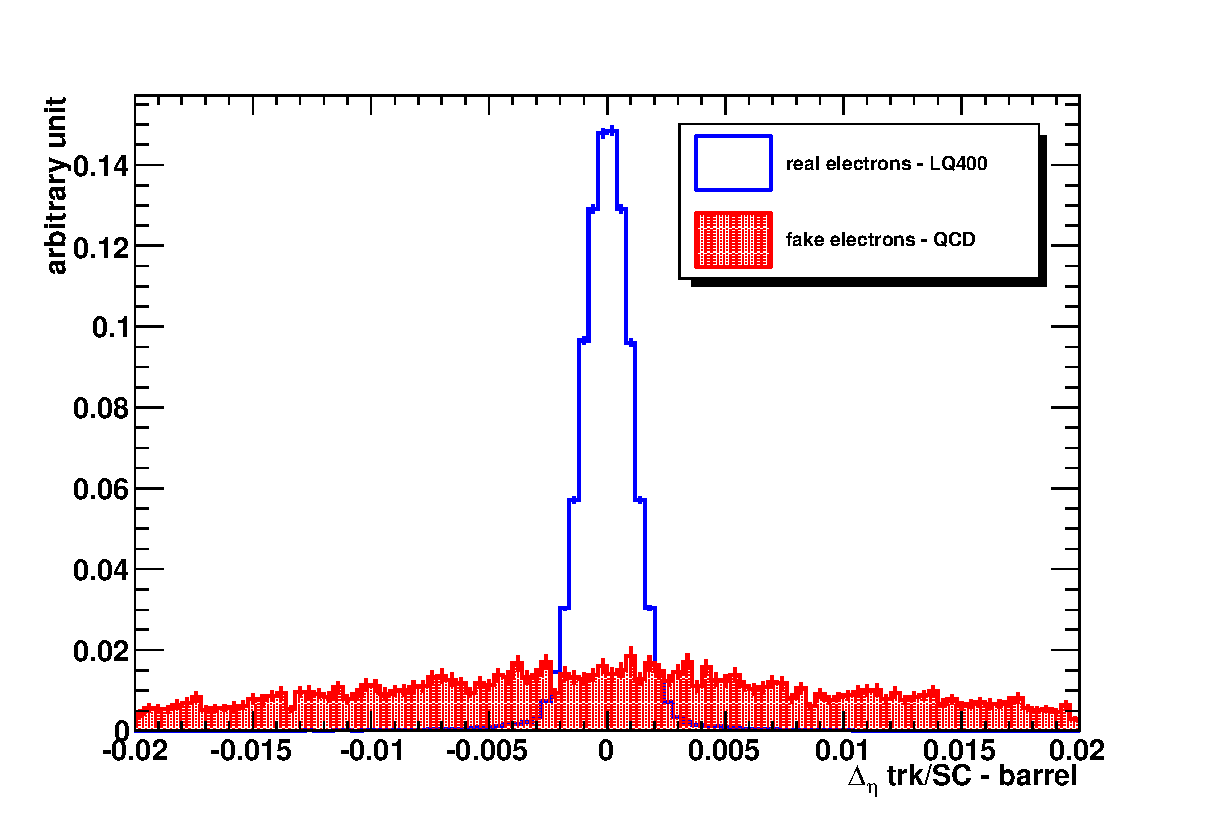
\includegraphics{plots/electronStudies/eleDeltaEtaTrkSC_barrel_LQ400vsQCD.eps}} &
  \resizebox{7cm}{!}{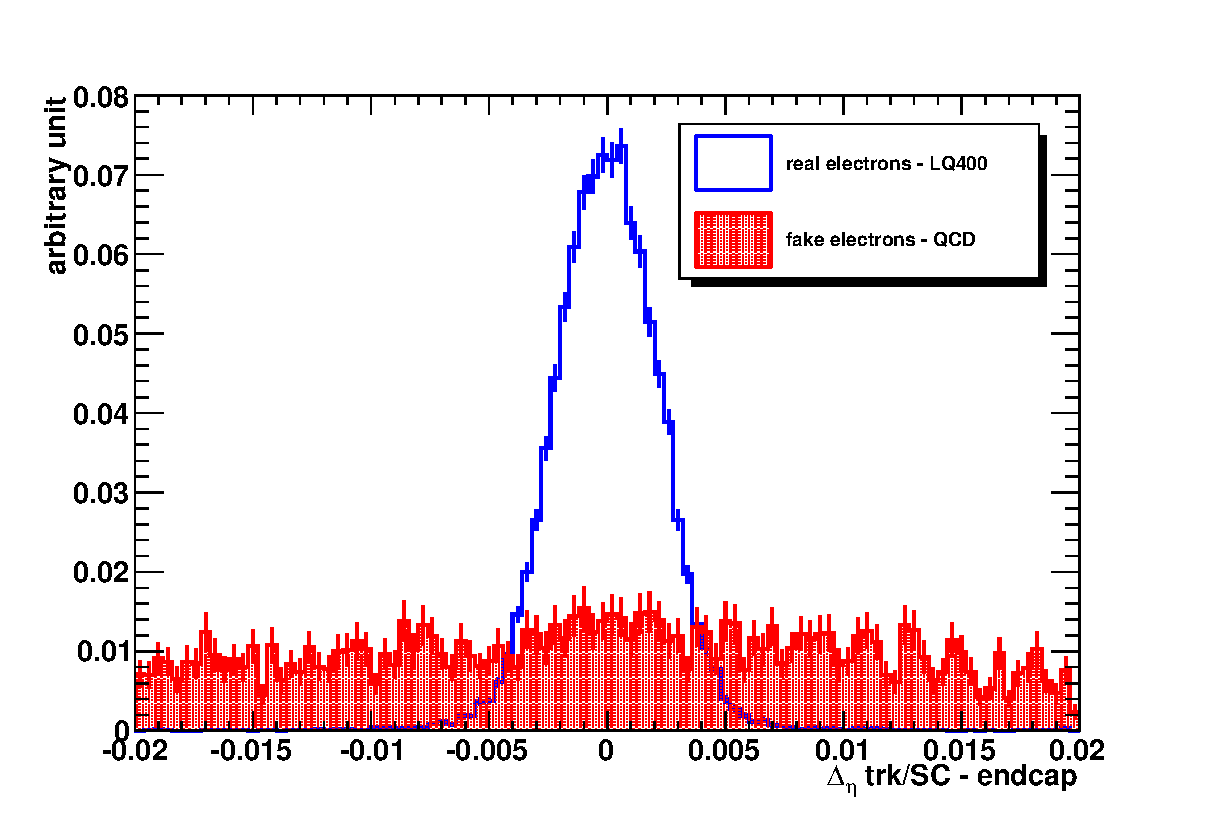
\includegraphics{plots/electronStudies/eleDeltaEtaTrkSC_endcap_LQ400vsQCD.eps}} \\
  \resizebox{7cm}{!}{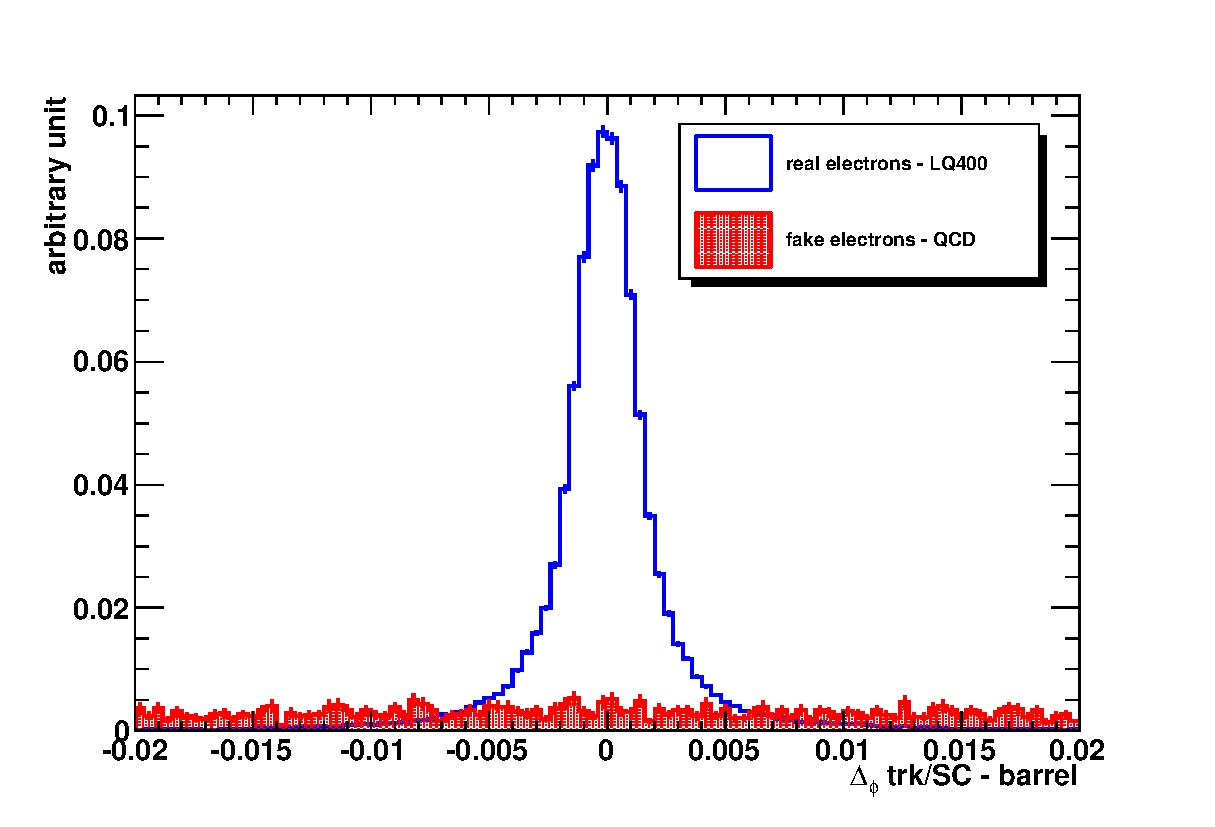
\includegraphics{plots/electronStudies/eleDeltaPhiTrkSC_barrel_LQ400vsQCD.eps}} &
  \resizebox{7cm}{!}{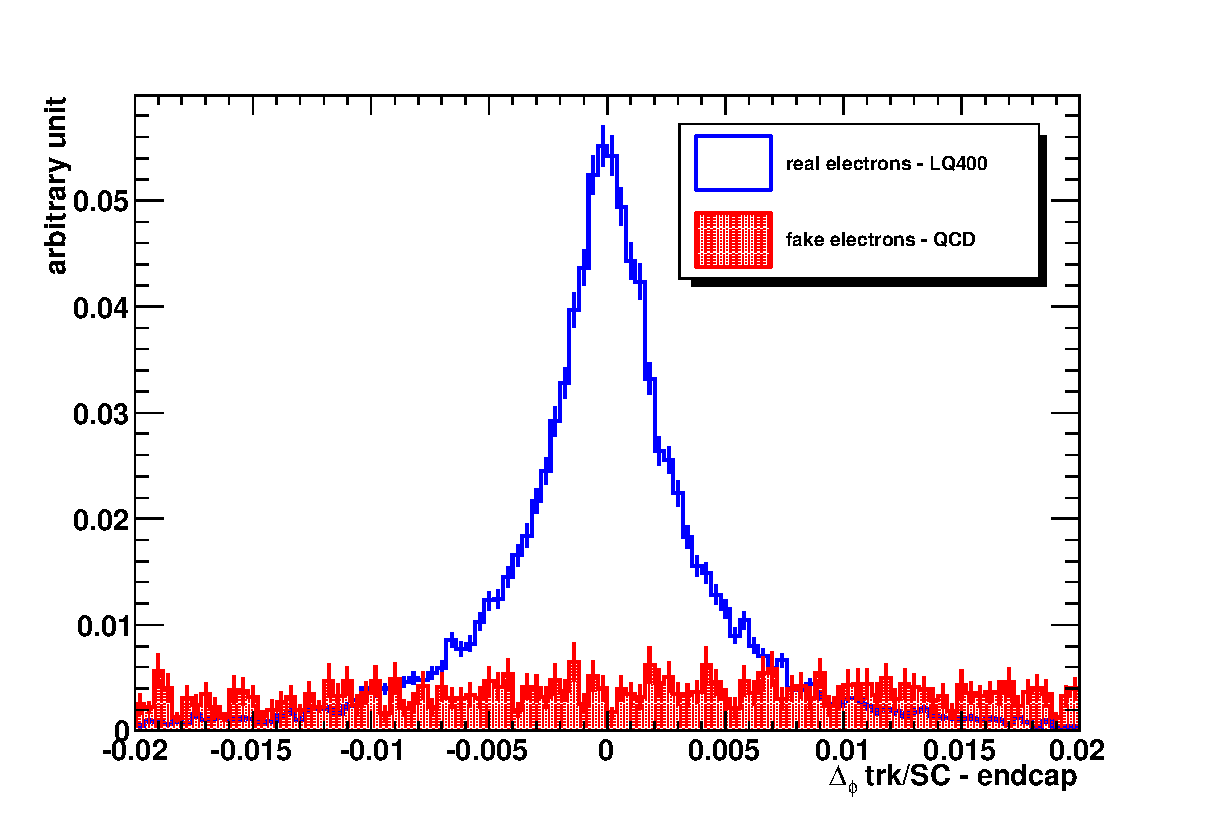
\includegraphics{plots/electronStudies/eleDeltaPhiTrkSC_endcap_LQ400vsQCD.eps}} \\
  \end{tabular} 
  \caption{\small \sl Distribution of electron-ID variables for true electrons from the decay of 400 GeV mass LQ, and false electrons from 
 QCD multi jets MC events. Electrons from LQ decay with generated $p_{T}>30$ GeV and $|\eta|<2.5$ are matched with reconstructed electrons with 
 $p_{T}>30$ GeV and $|\eta|<2.5$ if $\Delta$R between them is $<0.07$. Reconstructed electrons are associated to the 
 barrel (endcaps) if $|\eta|<1.442$ ($1.560<|\eta|<2.5$).}
 \label{fig:elecID}
  \end{center}
\end{figure}

\begin{figure}
  \begin{center}
  \begin{tabular}{cc}
  \resizebox{7cm}{!}{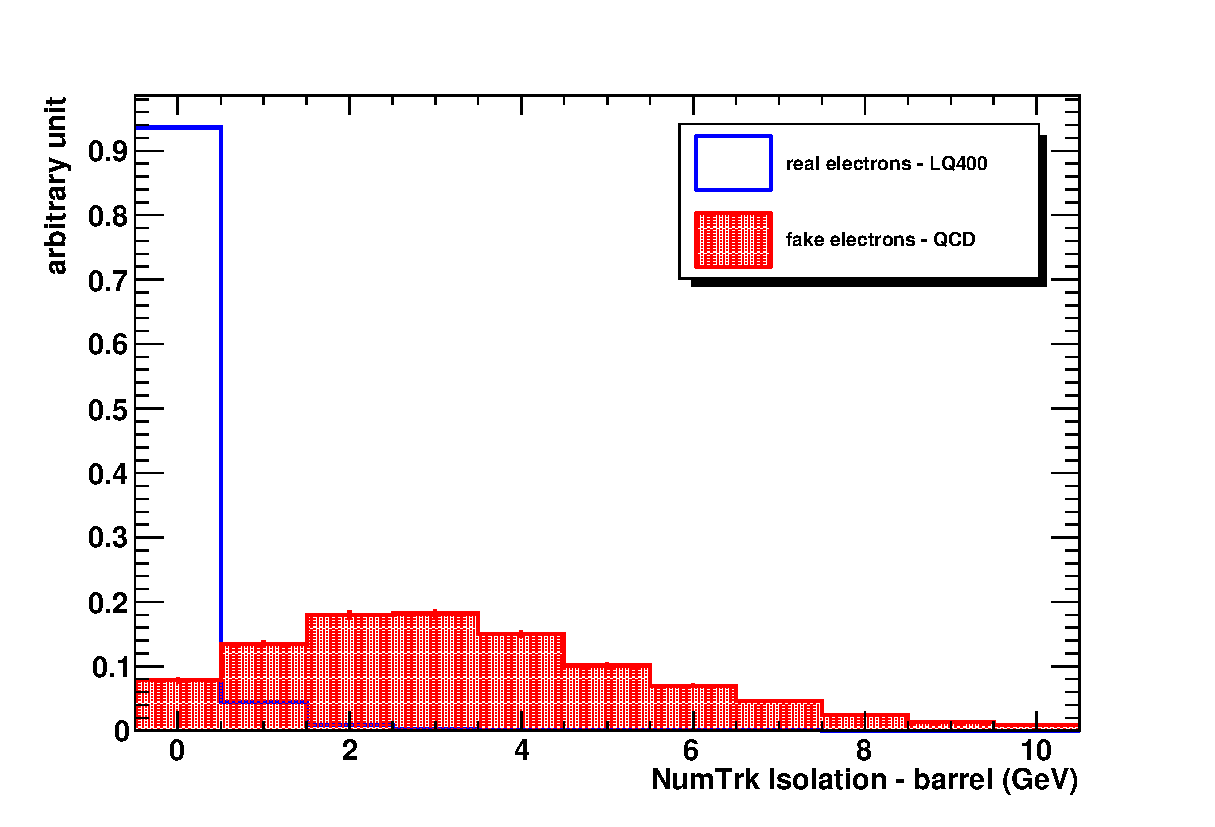
\includegraphics{plots/electronStudies/eleNumTrkIso_barrel_LQ400vsQCD.eps}} &
  \resizebox{7cm}{!}{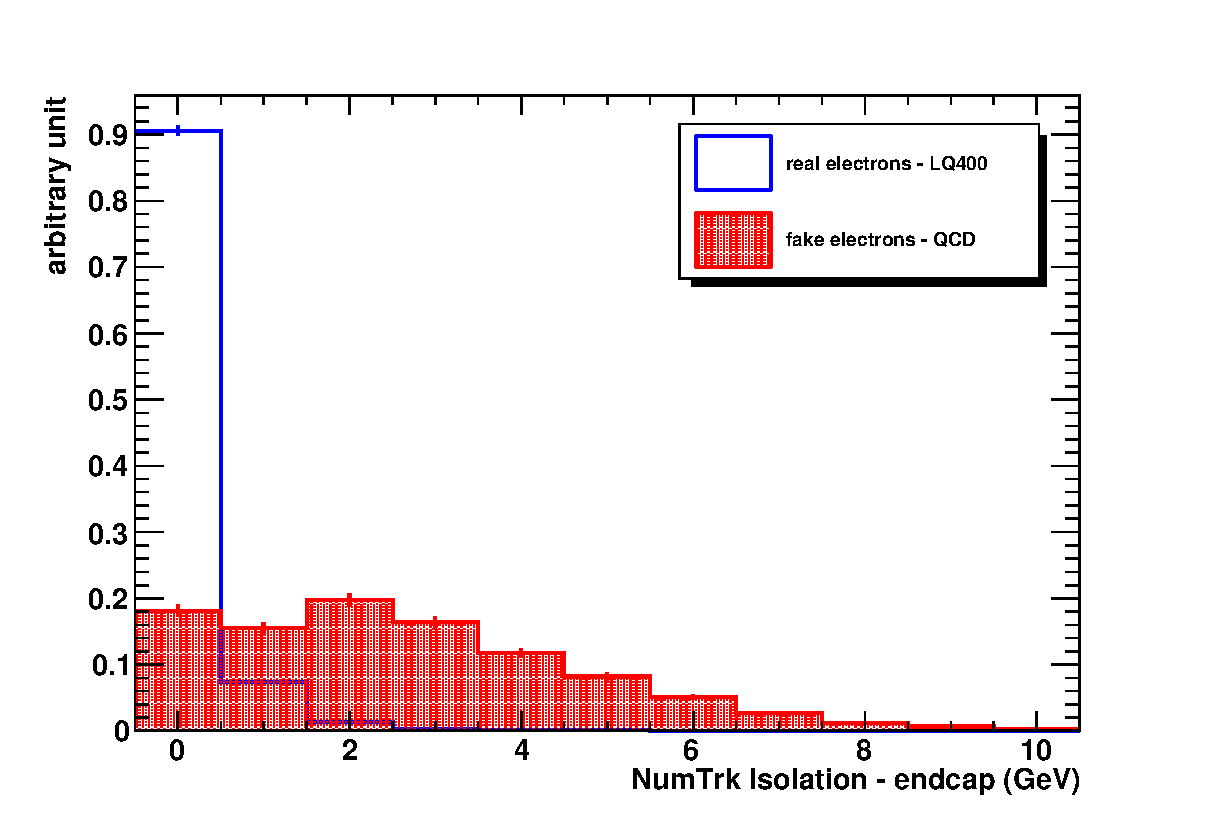
\includegraphics{plots/electronStudies/eleNumTrkIso_endcap_LQ400vsQCD.eps}}\\
  \resizebox{7cm}{!}{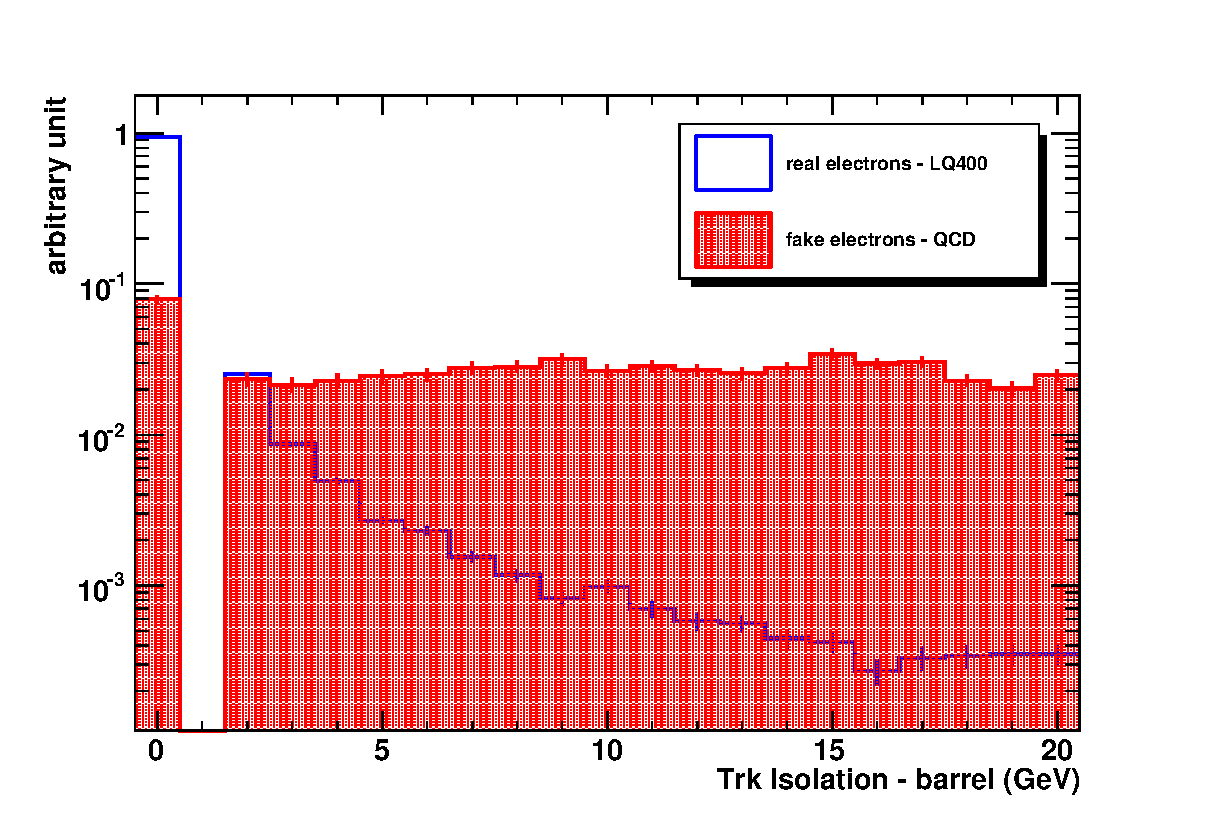
\includegraphics{plots/electronStudies/eleTrkIso_barrel_LQ400vsQCD.eps}} &
  \resizebox{7cm}{!}{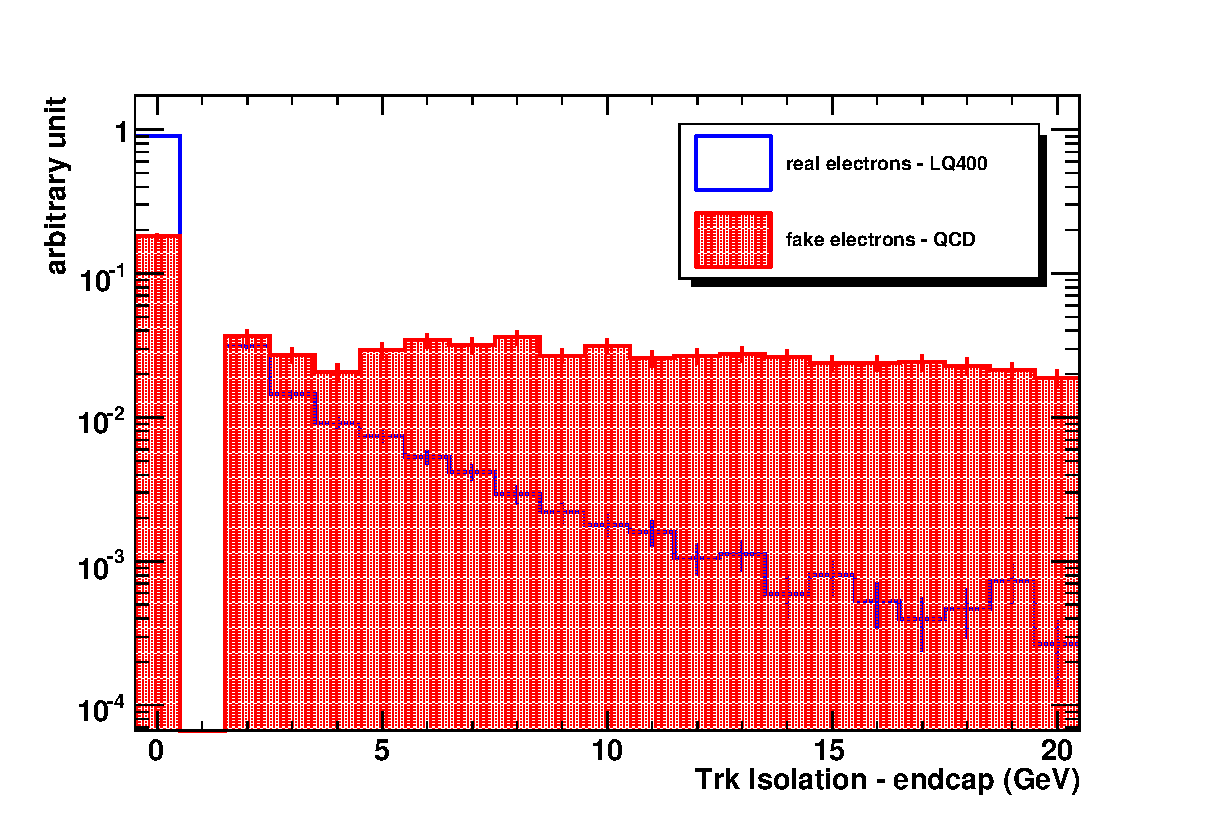
\includegraphics{plots/electronStudies/eleTrkIso_endcap_LQ400vsQCD.eps}} \\
  \resizebox{7cm}{!}{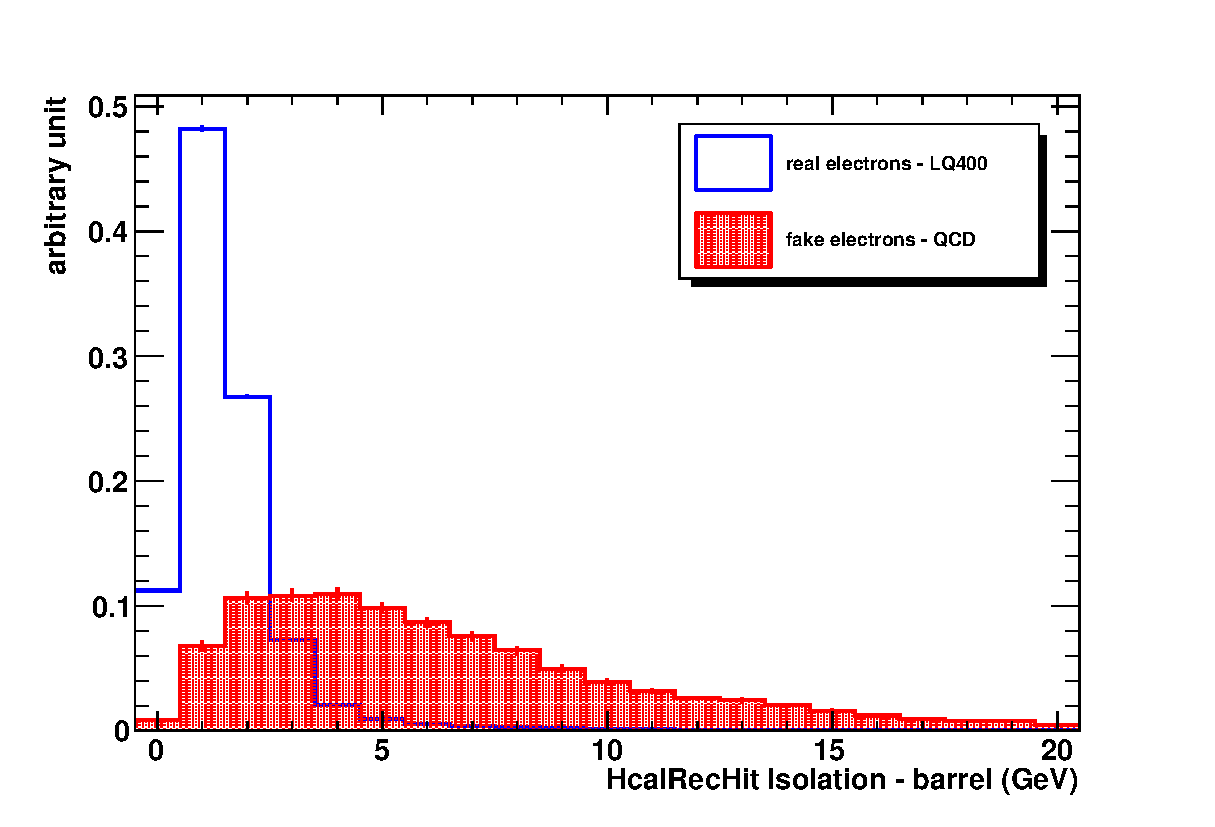
\includegraphics{plots/electronStudies/eleHcalRecHitIso_barrel_LQ400vsQCD.eps}} &
  \resizebox{7cm}{!}{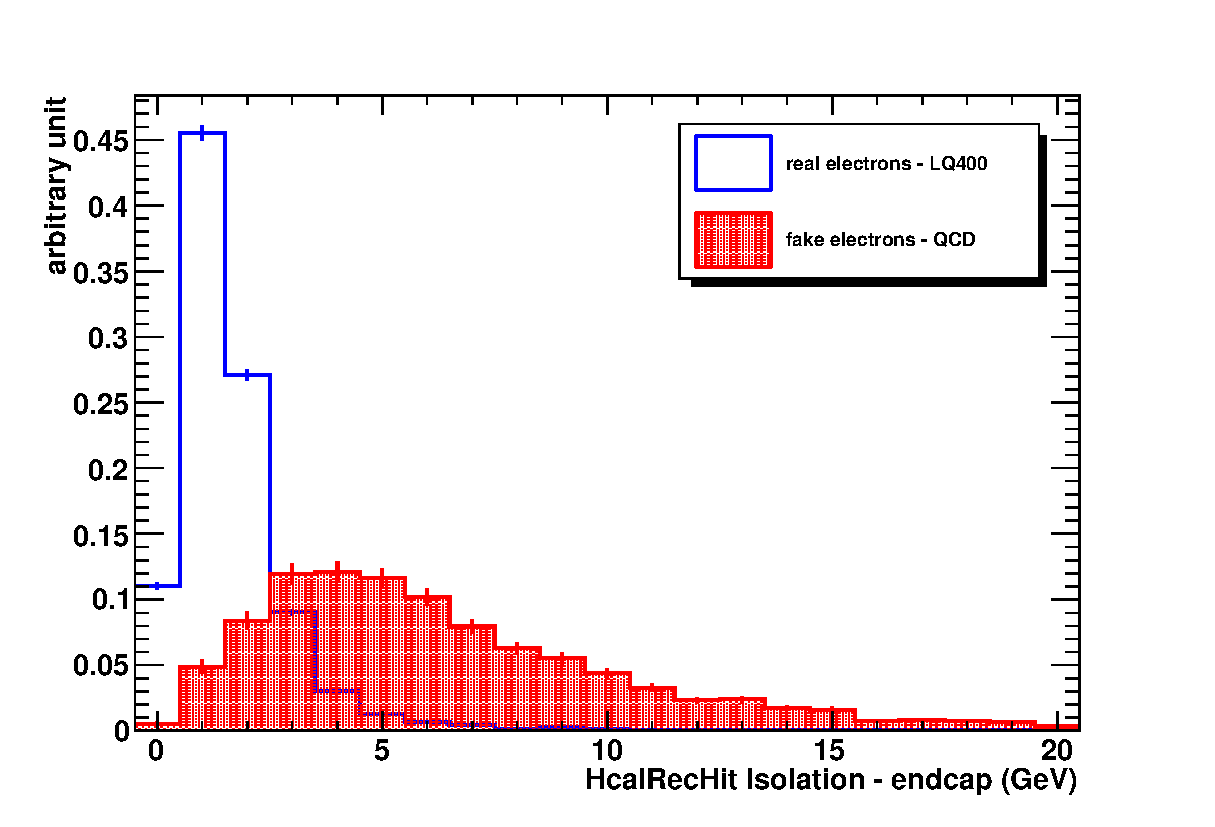
\includegraphics{plots/electronStudies/eleHcalRecHitIso_endcap_LQ400vsQCD.eps}} \\
  \resizebox{7cm}{!}{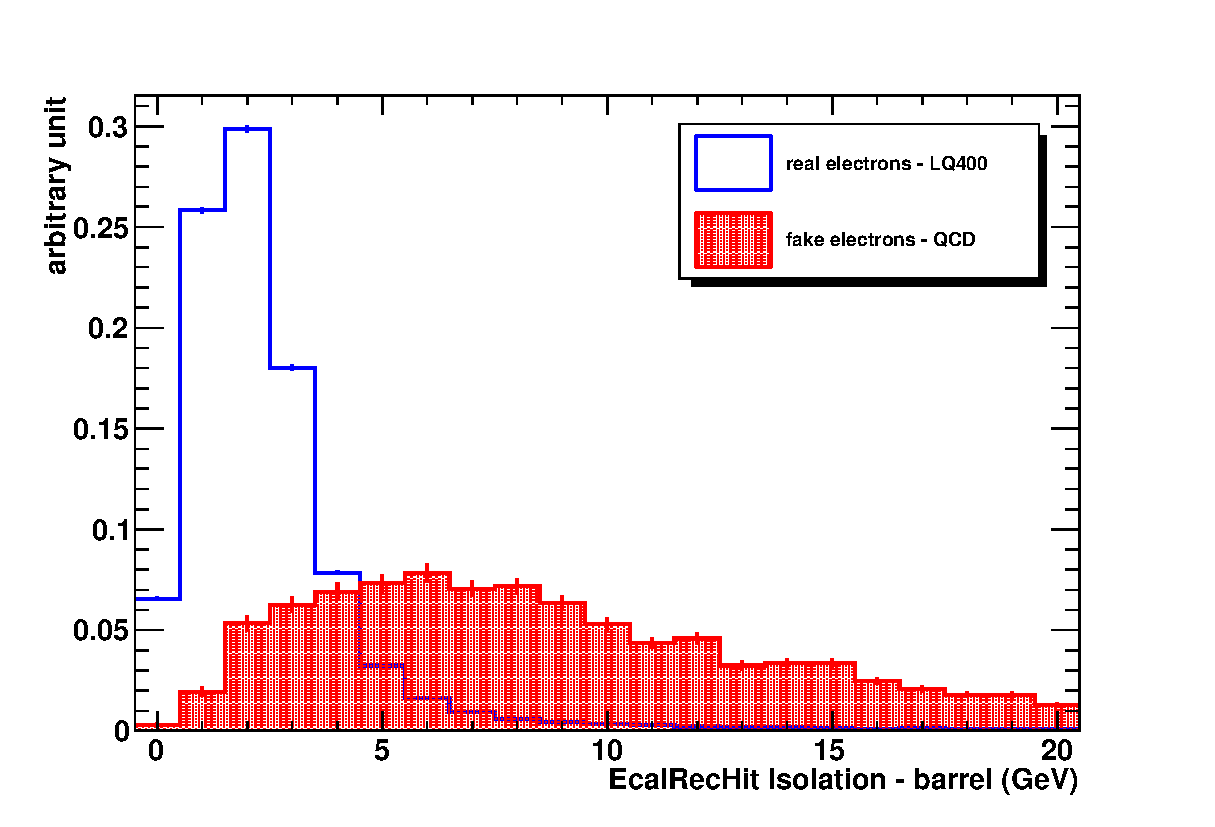
\includegraphics{plots/electronStudies/eleEcalRecHitIso_barrel_LQ400vsQCD.eps}} &
  \resizebox{7cm}{!}{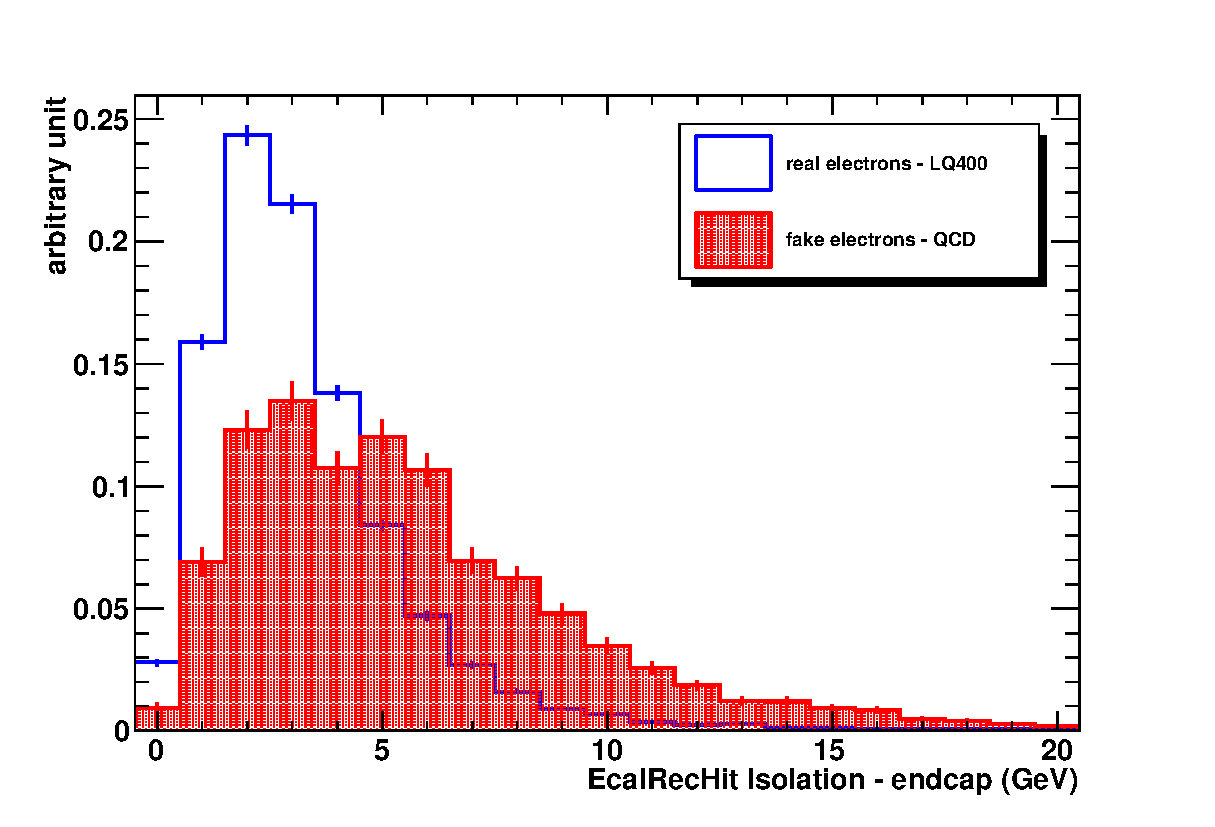
\includegraphics{plots/electronStudies/eleEcalRecHitIso_endcap_LQ400vsQCD.eps}} \\
  \end{tabular}
  \caption{\small \sl Distribution of electron-isolation variables for true electrons from the decay of 400 GeV mass LQ, and false electrons from 
    QCD multi jets MC events. Electrons from LQ decay with generated $p_{T}>30$ GeV and $|\eta|<2.5$ are matched with reconstructed electrons with 
    $p_{T}>30$ GeV and $|\eta|<2.5$ if $\Delta$R between them is $<0.07$. Reconstructed electrons are associated to the 
    barrel (endcaps) if $|\eta|<1.442$ ($1.560<|\eta|<2.5$).}
    \label{fig:elecIso}
  \end{center}
\end{figure}

\begin{table}[htbp]
  \label{tab:HEEPselection}
  \begin{center}
    \begin{tabular}{|lcc|lcc|} \hline
      \multicolumn{3}{|c|}{ID Variables} & \multicolumn{3}{|c|}{Isolation Variables} \\ 
      Variable & Barrel & Endcap & Variable & Barrel & Endcap  \\ \hline
      $H/E$  & $<0.05$ & $<0.1$ & $N_T$  & $<4$ & $<4$ \\ \hline
      $\sigma_{\eta\eta}$  & $<0.011$ & $<0.0275$ & Track Iso (GeV) & $<7.5$ & $<15$ \\ \hline
      $|\Delta\eta^{trk-SC}|$ & $<0.005$ & $<0.007$ & EM Iso (GeV) & $<6+0.01*E_{t}$ & $<6+0.01*E_{t}$ \\ \hline
      $|\Delta\phi^{trk-SC}|$ & $<0.09$ & $<0.09$ & HAD Iso (GeV) & $<4+0.005*E_{t}$ & $<4+0.005*E_{t}$ \\ \hline
    \end{tabular}
  \caption{\small \sl HEEP electron ID and isolation criteria. Reconstructed electrons are associated to the 
    barrel (endcaps) if $|\eta|<1.442$ ($1.560<|\eta|<2.5$).}
  \end{center}
\end{table}


\subsection{Acceptance and Reconstruction Efficiency} \label{sec:electronEfficiency}

Electrons from LQ decays, being usually isolated from jets and having a $p_{T}$ of 
hundreds of GeV, can be reconstructed with high efficiency. 
Table~\ref{tab:ElecEffAcc}
shows the electron acceptance $A_{gen}$
(the acceptance cuts are $p_{T}^{gen}>$ 30 $GeV/c$ and $|\eta^{gen}|<2.5$),
the efficiency, $\varepsilon_{ele}$, for a reconstructed electron that have passed ID and isolation requirements
within the acceptance region, and the overall efficiency, $A_{gen} \times \varepsilon_{ele}$,
for single electrons from LQ decays for a 400 $GeV/c^2$ LQ mass.
The overall single electron efficiency, including acceptance, is $\approx 80\%$.

Figure~\ref{fig:elecEffFV} shows the reconstruction, ID and isolation efficiencies
(within the acceptance region) of electrons for LQ mass of 400 GeV as a function of electron $\eta$ and $p_{T}$. 
A significant loss of efficiency is seen in the region $|\eta| \approx 1.5$, 
and is due to the lack of calorimeter coverage between the ECAL barrel and the endcaps. 
The inefficiency at high $|\eta|$ is a border effect related to the 
geometrical acceptance of the inner tracking system, that ends at $|\eta| = 2.5$.
Once real data is available, electron efficiencies will be measured 
with $tag\&probe$ method using $Z \rightarrow ee$ events 
following the approach discussed at~\cite{TagAndProbe}. \\

%
\begin{table}[htb]
  \begin{center}
    \begin{tabular}{|l|c|c|c|} \hline
      LQ mass (GeV) & $A_{gen}$ & $\varepsilon_{ele}$ & $A_{gen} \times \varepsilon_{ele}$\\ \hline
      400 & 96.4\% & 83.4\% & 80.4\% \\ \hline
    \end{tabular}
    \caption{\small \sl Electron acceptance ($A_{gen}$), 
      reconstruction efficiency after ID and isolation cuts ($\varepsilon_{ele}$), and overall reconstruction efficiency 
      ($A_{gen} \times \varepsilon_{ele}$) for single electrons from decays of LQ with mass of 400 GeV (FullSim sample used).   
      Relative statistical uncertainties on efficiencies are less than 0.2\%.  
      } 
  \end{center}
  \label{tab:ElecEffAcc}
\end{table}
%
\begin{figure}
  \begin{center}
  \begin{tabular}{cc}
    \resizebox{8.2cm}{!}{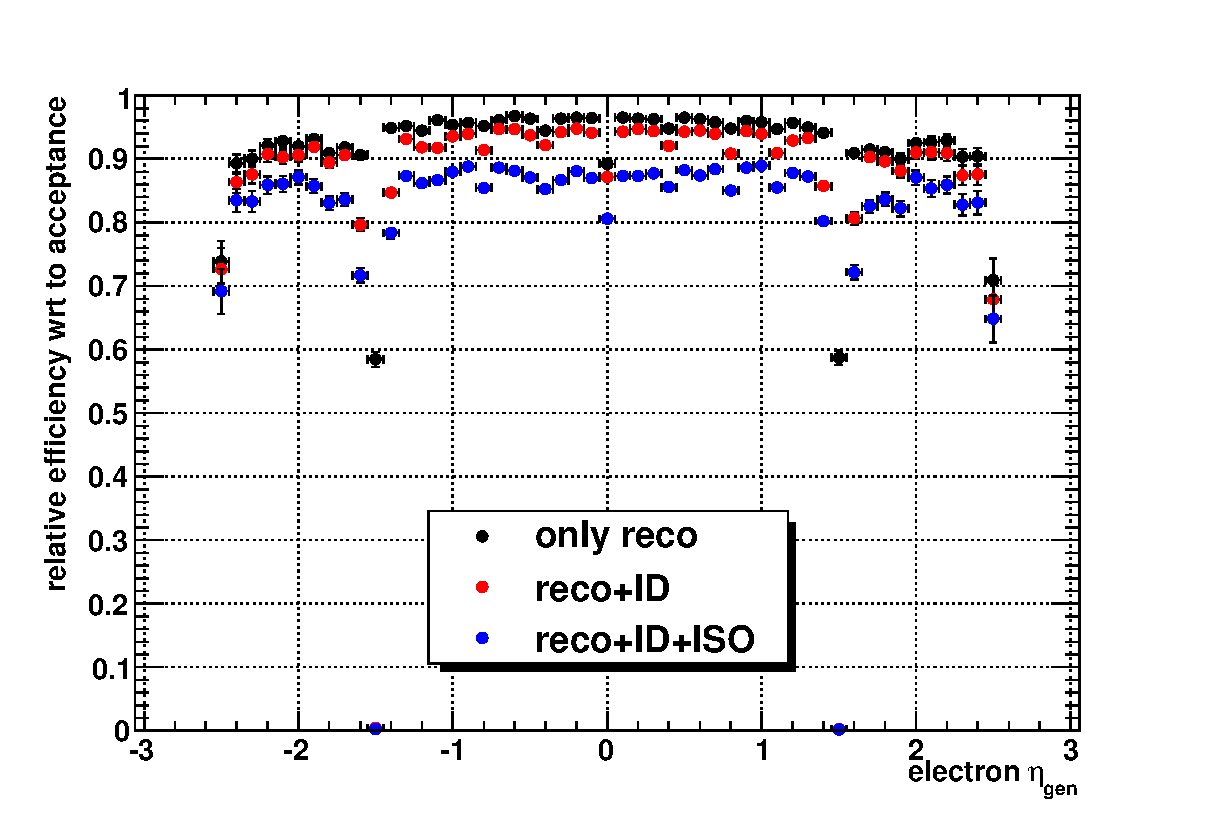
\includegraphics{plots/electronStudies/Eff_vs_Eta_recoIDIsoEle_pT30_eta2.5_LQ400.eps}} &
    \resizebox{8.2cm}{!}{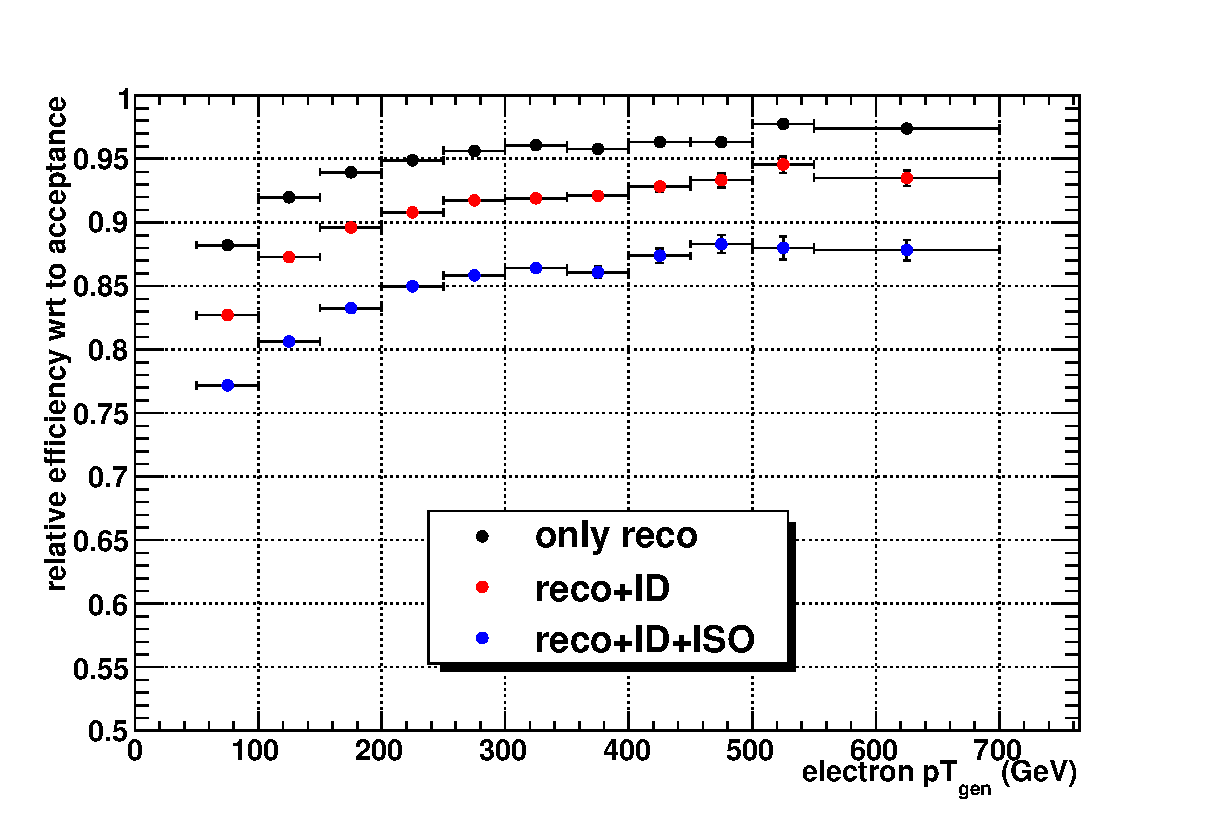
\includegraphics{plots/electronStudies/Eff_vs_pT_recoIDIsoEle_pT30_eta2.5_LQ400.eps}} \\
    \end{tabular}
    \caption{\small \sl Electron reconstruction, ID and isolation efficiency as a function of electron $\eta^{gen}$ and $p_{T}^{gen}$. 
      A FullSim sample of LQ with mass of 400 GeV is used.}
  \end{center}
  \label{fig:elecEffFV}
\end{figure}
%

% indico.cern.ch/getFile.py/access?contribId=3&resId=0&materialId=slides&confId=32048


%\begin{figure}
%  \begin{center}
%  \begin{tabular}{c}
%    %\resizebox{9cm}{!}{\includegraphics{plots/Ele_eff_M650GeV.eps}}
%    \resizebox{10cm}{!}{
\includegraphics{plots/UMD.eps}} \\
%    \resizebox{10cm}{!}{
\includegraphics{plots/UMD.eps}} \\ 
%%  \resizebox{5cm}{!}{
\includegraphics{plots/UMD.eps}} &
%%  \resizebox{5cm}{!}{
\includegraphics{plots/UMD.eps}} \\
%  \end{tabular}
%  \caption{\small \sl Distributions of some reconstructed quantities for electrons from LQ decay, 
%    obtained with FastSim (blue filled histogram) and FullSim (black dots) 
%    samples with $M_{LQ}=650$ GeV.
%    From the top-left to the bottom-right: $p_{T}$, $\eta$, $\Delta\phi_{in}$, $\Delta\eta_{in}$.}
%  \label{fig:elecVariables}
%  \end{center}
%\end{figure}

%efficiency (pT, eta) (no deltaR from genJet since already showed distance OK above)
%pT, eta dist
%{\Large \sl Energy Resolution}
%fast vs full

%\end{document}
